\documentclass[slidestop,compress,red,notes,xcolor=dvipsnames]{beamer}	%L'opzione xcolor semplifica la nomenclatura dei colori

\usepackage[italian]{babel}
\usepackage{hyperref}
\usepackage[utf8]{inputenc}
%\usepackage[bars]{beamerthemetree}

\title{OpenStreetMap\\\textit{Una mappa libera per il nostro Pianeta}}
\author{Francesco de Virgilio - Alessandro De Noia}
\institute{LUGBari - LinuxDay 2008}
\date{\today}

\usetheme{Warsaw}
\setbeamertemplate{footline}{}				%Questa riga elimina la footline in fondo alla pagina (i nomi degli autori non ci entrano tutti)
\setbeamercolor{section in head/foot}{bg=BurntOrange}	%Questa riga e quella successiva gestiscono i due colori della presentazione
\setbeamercolor{subsection in head/foot}{bg=RawSienna}	%
\useoutertheme{shadow}
\useinnertheme{rounded}
\usecolortheme{structure} 
\beamertemplateshadingbackground{blue!5}{green!10}	%Sfondo della diapositiva
\beamertemplatetransparentcovereddynamicmedium		%Rende semitrasparenti gli elementi non visualizzati delle liste con pause

%%%% CC %%%%
\input{cc_beamer}

%%%% LOGO %%%%
\logo{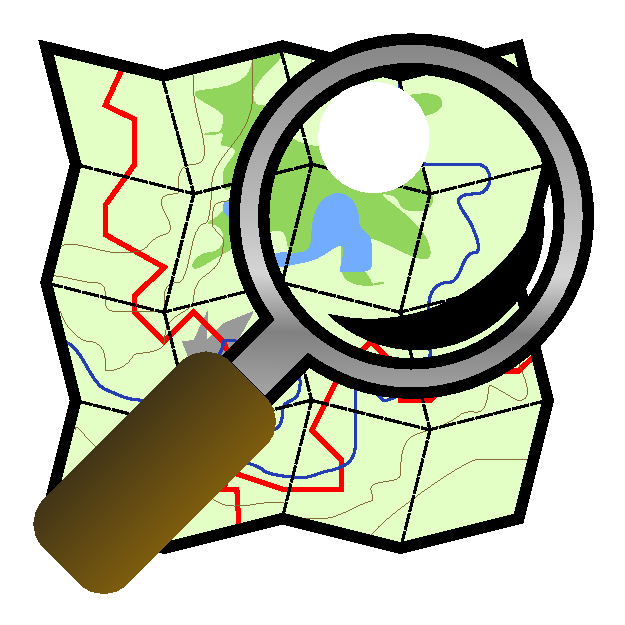
\includegraphics[height=1.2cm]{images/logo.eps}}		%Inserisce il logo in ogni slide

\begin{document}
\frame{\titlepage}

\section{Introduzione}

    \begin{frame}{Cos'è OpenStreetMap?}
        \begin{center}
            OpenStreetMap è un progetto che punta a \textbf{creare} e \textbf{fornire} dati cartografici liberi e gratuiti a chiunque ne abbia bisogno; questi dati vengono usati per creare una mappa collaborativa del Pianeta.
        \end{center}
        \pause
        \begin{block}{Perchè OpenStreetMap?}
            Il progetto è stato lanciato perché la gran parte delle mappe che potresti pensare essere gratuite, hanno invece - oltre a frequenti errori - \textbf{restrizioni legali o tecniche al loro uso}, impedendo alle persone il loro uso per scopi produttivi, creativi ed altri.
        \end{block}
     \end{frame}

    \begin{frame}{Cos'è OpenStreetMap?}
        \vspace{1cm}
        \begin{center}
            
\includegraphics[height=2cm]{images/wiki.eps}
        \end{center}
    \end{frame}

    \begin{frame}{Come appare una mappa di OpenStreetMap}
        \begin{center}
            \includegraphics[height=7cm]{images/Pinelands.eps}
        \end{center}
    \end{frame}

\section{La libertà}

    \begin{frame}
        \vspace{1.5cm}
        \begin{center}
            \begin{huge}
                \textbf{La Libertà delle Mappe}
            \end{huge}
        \end{center}
    \end{frame}

    \begin{frame}{La libertà delle mappe}
         In molti paesi i geodati e le mappe, pur essendo state finanziate dagli enti pubblici (e quindi con il denaro dei contribuenti), non vengono ``restituite'' ai cittadini permettendo loro l'utilizzo dei dati ma sono, al contrario, coperte da \textbf{copyright}; questi dati vengono poi ``rivenduti'' ai cittadini, che devono quindi pagare due volte per ottenere un unico servizio. OpenStreetMap ha l'obiettivo di collezionare geodati per la realizzazione di mappe che possano essere libere al punto che \textit{chiunque può usarle per i propri scopi}.\pause
         \begin{block}{Gli USA: un modello}
             Negli USA i geodati raccolti dagli enti pubblici sono liberamente disponibili con licenza di \textbf{Pubblico Dominio}.
         \end{block}
    \end{frame}

    \begin{frame}{``Ma io uso già Google Maps\ldots''}
        In generale, le mappe che si trovano su internet non sono libere, ma coperte da diritto d'autore, che ne limita o proibisce qualsiasi utilizzo non autorizzato; in questa situazione ricadono anche:
        \pause
        \begin{itemize}
            \item Google Maps
            \item Tom Tom
            \item Garmin
        \end{itemize}
        \pause
        Le mappe tradizionali:
        \begin{itemize}
            \item hanno errori fatti ad arte
            \item i dati sorgenti non sono disponibili
            \item non sono aggiornate/complete
            \item non si possono correggere
            \item non si possono rivendere/utilizzare per altri scopi
        \end{itemize}
    \end{frame}

    \begin{frame}{I vantaggi di OpenStreetMap}
        OpenStreetMap è una mappa in stile wiki, in cui chiunque può dare il proprio contributo, aggiungendo, modificando o eliminando strade, nomi, punti d'interesse, ecc.
        \begin{center}
            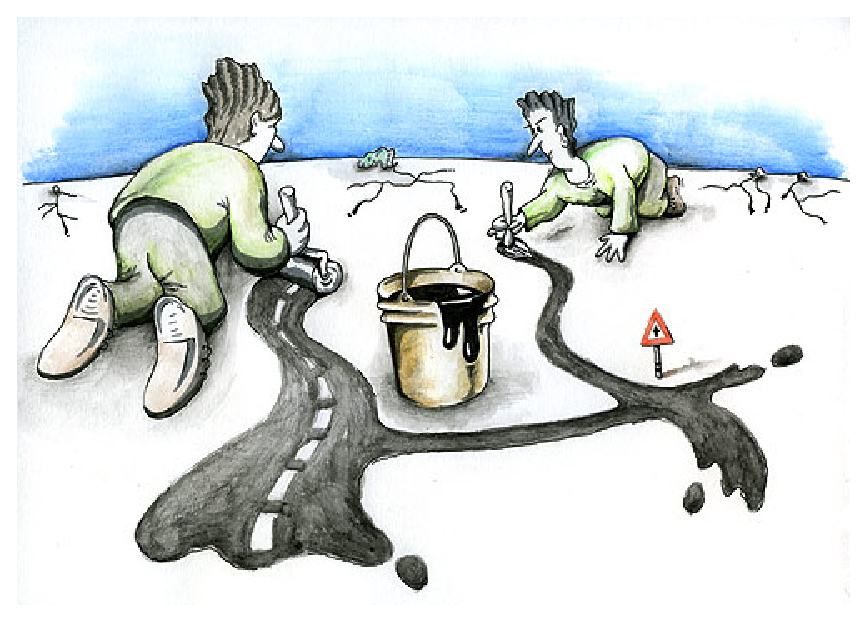
\includegraphics[height=3cm]{images/cartoon.eps}
        \end{center}
        Utilizzare una mappa in stile ``wiki'' significa avere:
        \pause
        \begin{itemize}
            \item Libertà
            \item Affidabilità
            \item Flessibilità
        \end{itemize}
    \end{frame}

    \begin{frame}{Libertà}
        Tutti i geodati e le mappe di OpenStreetMap sono rilasciati con licenza \textit{\textbf{Creative Commons Attribuzione - Condividi allo stesso modo 2.0}}
        \begin{center}
            
\includegraphics[height=1cm]{images/cc.eps}
        \end{center}
        Tutti abbiamo le seguenti libertà:
        \pause
        \begin{itemize}
            \item copiare le mappe
            \item modificare le mappe
            \item ridistribuire le mappe
            \item utilizzare per scopi commerciali le mappe
        \end{itemize}
        \pause
        Purchè
        \begin{itemize}
            \item sia citata la fonte di dati/mappe (OpenStreetMap)
            \item qualunque creazione derivata deve essere rilasciata sotto la stessa licenza
        \end{itemize}
    \end{frame}

    \begin{frame}{Affidabilità}
        Le mappe di OpenStreetMap sono \textbf{prive di \textit{easter eggs}}, errori inseriti volutamente per riconoscere le mappe copiate.\\ \vspace{0.5cm}
        \textit{Sutton coldfield, Regno Unito; Warvick Road non esiste!}
        \begin{center}
            \includegraphics[height=4cm]{images/geo_map.eps}
        \end{center}
    \end{frame}

    \begin{frame}{Flessibilità}
        I dati di OpenStreetMap possono essere usati in molte maniere diverse, principalmente per creare mappe; le mappe possono essere trasferite, copiate e modificate per qualsiasi scopo.\\ Vediamo alcuni esempi:
    \end{frame}

    \begin{frame}{Navigatori GPS}
        \textbf{Garmin eTrex}...\\
        \begin{center}
            \includegraphics[height=6cm]{images/nav_gps.eps}
        \end{center}
    \end{frame}

    \begin{frame}{In auto}
        \textbf{...nel cruscotto...}\\
        \begin{center}
            \includegraphics[height=5.5cm]{images/car.eps}
        \end{center}
    \end{frame}

    \begin{frame}{Online Routing}
        \textbf{...online...}
        \begin{center}
            \includegraphics[height=5cm]{images/route.eps}
        \end{center}
    \end{frame}

    \begin{frame}{Videogames}
        \textbf{...nei giochi: \textit{FlightGears}...}
        \begin{center}
            \includegraphics[height=6cm]{images/gears.eps}
        \end{center}
    \end{frame}

    \begin{frame}{Sui palmari}
        \textbf{...nel palmo della mano...}\\
        \vspace{1cm}
        \includegraphics[height=3.5cm]{images/nokia.eps}
        \includegraphics[height=3.5cm]{images/bike.eps}
    \end{frame}

    \begin{frame}{Nel telefonino}
        \textbf{...negli smartphones...}\\
        \begin{center}
            \includegraphics[height=6cm]{images/tango.eps}\hspace{1cm}
            \includegraphics[height=6cm]{images/cell.eps}
        \end{center}
    \end{frame}

    \begin{frame}{Su carta}
        \textbf{...finalmente la cartina!}\\
        \begin{center}
            \includegraphics[height=6.5cm]{images/mappa.eps}
        \end{center}
    \end{frame}

    \section{Come funziona}

        \begin{frame}{Come funziona}
        \vspace{1.5cm}
        \begin{huge}\begin{center}\textbf{Come funziona?} \end{center}\end{huge}
        \end{frame}

        \begin{frame}{Le fasi}
            Il mapping è diviso in 3 fasi:
            \pause
            \begin{itemize}
                \item Raccolta dati
                \begin{itemize}
                    \item dinamica: il GPS
                    \item statica: Yahoo! Aerial 
                \end{itemize}
                \vspace{0.5cm}
                \pause
                \item Editing dei dati
                \begin{itemize}
                    \item disegnare le strade
                    \item inserire altri dati
                \end{itemize}
                \vspace{0.5cm}
                \pause
                \item Rendering
                \begin{itemize}
                    \item Mapnik, il render ``ufficiale''
                    \item Osmarender, il render ``veloce''
                \end{itemize}
            \end{itemize}
        \end{frame}

        \begin{frame}{Mapping dinamico: il GPS}
            Con un ricevitore GPS (telefonino, palmare, navigatore da auto) è possibile ``registrare'' le tracce delle strade percorse.\pause\\
            Accorgimenti:
            \begin{itemize}
                \item attendere il fix di almeno 5 satelliti
                \pause
                \item palazzi alti ed altre strutture possono far deviare il tracciato gpx
                \pause
                \item il segnale può scomparire o non essere ottimale in gallerie, sottopassi o lunghi ponti
            \end{itemize}
        \end{frame}

        \begin{frame}{Mapping dinamico: il GPS}
            Raccolta di tracce gpx...
            \vspace{1cm}
            \begin{center}
                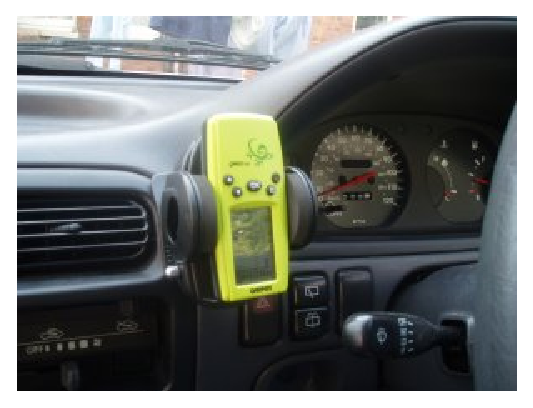
\includegraphics[height=4cm]{images/auto.eps}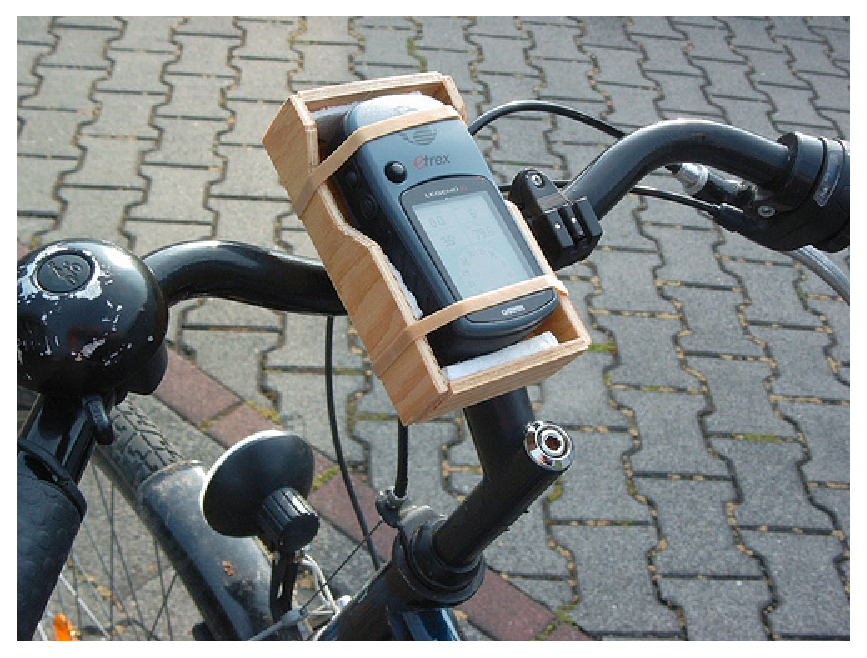
\includegraphics[height=4cm]{images/grezzata.eps}
            \end{center}
        \end{frame}

        \begin{frame}{Mapping dinamico: il GPS}
            Raccolta di tracce gpx...
            \begin{center}
                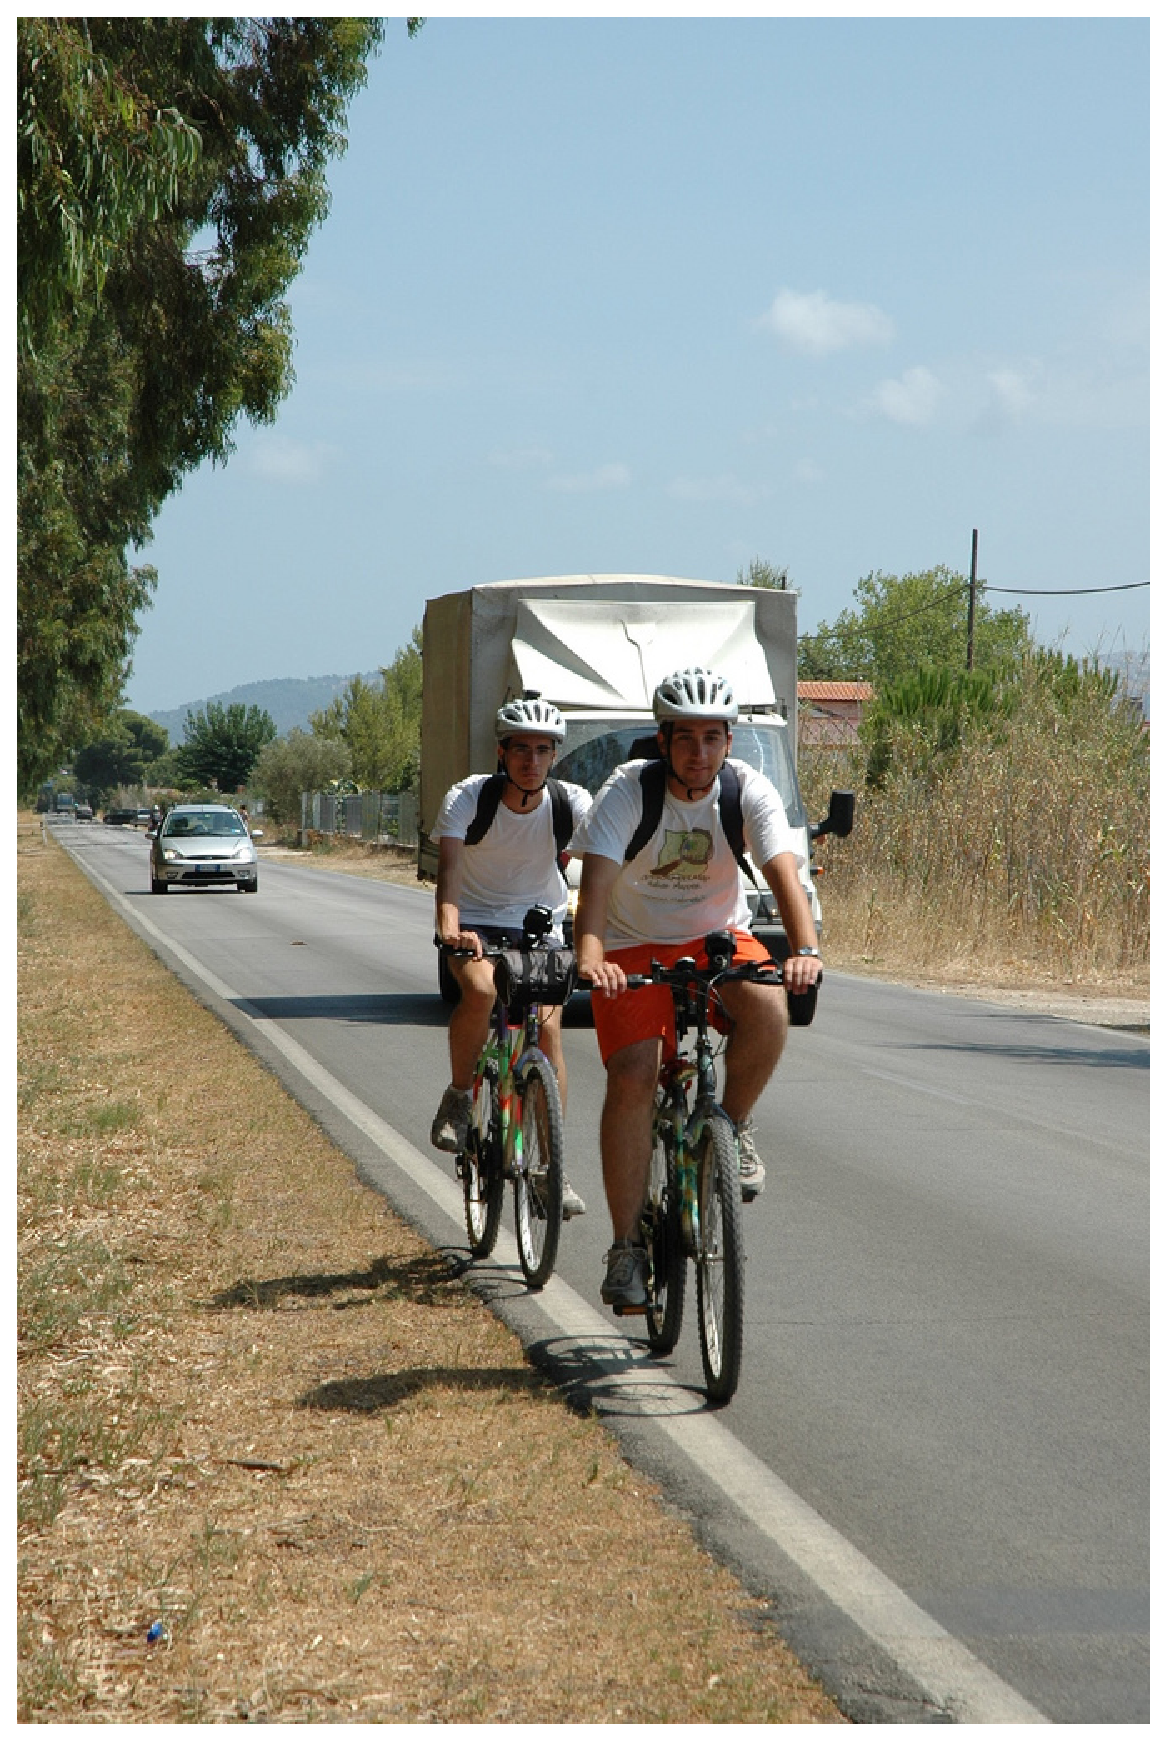
\includegraphics[height=6.5cm]{images/bici.eps}
            \end{center}
        \end{frame}

        \begin{frame}{Mapping dinamico: il GPS}
            Oltre alle tracce gpx, si possono raccogliere le coordinate di altri elementi interessanti lungo il percorso:
            \begin{itemize}
                \item nomi delle vie
                \item sensi unici e divieti d'accesso
                \item semafori
                \item fermate dell'autobus
                \item strisce pedonali
                \item dossi
                \item autovelox
                \item punti di raccolta materiali riciclabili
                \item e diverse decine di altri elementi...
            \end{itemize}
        \end{frame}

        \begin{frame}{Mapping dinamico: il GPS}
            Per raccogliere questi elementi, è possibile aiutarsi con
            \pause
            \begin{itemize}
                \item taccuino (su cui disegnare strade, nomi e punti interessanti)
                \pause
                \item registratore
                \pause
                \item macchina fotografica
            \end{itemize}
            \pause
            \begin{block}{Georeferenziazione foto/audio}
                Se l'orologio della macchina fotografica o del registratore è sincronizzato con l'ora UTC del GPS, è possibile (tramite programmi di gestione delle fotografie come Digikam) georeferenziare le fotografie e l'audio, per disegnare più velocemente le mappe in editor che supportano la visualizzazione di foto/audio georeferenziati (JOSM).
            \end{block}
        \end{frame}

        \begin{frame}{Mapping statico: Yahoo! Aerial Maps}
        \textbf{Potlatch:}
            \begin{itemize}
                \item editor online in Flash
                \pause
                \item disponibile una modalità ``Play'' per principianti
                \pause
                \item apprendimento veloce e layout intuitivo
                \pause
                \item ottimo per piccole modifiche o mapping da \textit{Yahoo! Aerial Maps}
                \pause
                \item funzionalità limitate
                \pause
                \item utilizzabile solo online
                \pause
                \item visualizza solo gpx precedentemente caricati
            \end{itemize}
        \end{frame}

        \begin{frame}{Mapping statico: Yahoo! Aerial Maps}
            Seduti in poltrona... \textbf{Potlatch!}
            \begin{center}
                \includegraphics[height=6cm]{images/pot.eps}
            \end{center}
        \end{frame}

        \begin{frame}{Editing dei dati}
            Dopo l'upload dei gpx, è possibile usare indistintamente Potlatch (online) o JOSM (offline)\pause\\
            \vspace{0.4cm}
            \textbf{JOSM} (Java OpenStreetMap \begin{footnotesize}Editor\end{footnotesize}):
            \begin{itemize}
                \item editor offline in Java (multipiattaforma)
                \pause
                \item è possibile fare pratica senza fare l'upload dei dati
                \pause
                \item ottimo per lavoro ``tecnico'', modifiche dettagliate, o di grandi dimensioni
                \pause
                \item ampie funzionalità
                \begin{itemize}
                    \item foto georiferite
                    \item audio georiferito
                    \item liveGPS
                    \item validazione upload
                    \item altri strumenti utili...
                \end{itemize}
                \pause
                \item apprendimento lento
            \end{itemize}
        \end{frame}

        \begin{frame}{Editing dei dati}
            \begin{center}
                \includegraphics[height=7cm]{images/josm1.eps}
            \end{center}
        \end{frame}

        \begin{frame}{Editing dei dati}
            \begin{center}
            \includegraphics[height=7cm]{images/josm2.eps}
            \end{center}
        \end{frame}

        \begin{frame}{Editing dei dati}
            Flusso di lavoro con JOSM:
            \begin{itemize}
                \item aprire una traccia gpx o inquadrare una zona di lavoro
                \item scaricare il layer gpx
                \item scaricare il layer dati
                \item editing del layer dati
                \item upload dei dati modificati con eventuale risoluzione dei conflitti
            \end{itemize}
        \end{frame}

        \begin{frame}{Editing dei dati}
            Il mondo secondo JOSM:
            \begin{itemize}
                \item la strada è una sequenza di nodi: \textit{way}
                \item un singolo nodo è usato per indicare singole entità (statue, fontane, semafori)
                \item una sequenza di nodi chiusi può individuare un elemento più grande o un'area
                \item le proprietà di nodi e sequenze di nodi vengono specificate tramite i \textit{tag}
            \end{itemize}
        \end{frame}

        \begin{frame}{Rendering}
            \begin{large}
                \textbf{Mapnik, il render ``ufficiale'':}
            \end{large}\\
            La mappa principale è generata ogni mercoledì sera dal dump settimanale del planet.osm. È visitabile su www.openstreetmap.org. Include i seguenti layer:
            \begin{itemize}
                \item Mapnik
                \item Osmarender
                \item CycleMap
                \item NoName
            \end{itemize}
        \end{frame}

        \begin{frame}{Rendering}
            \begin{large}
                \textbf{Osmarender, il render ``veloce'':}
            \end{large}\\
            La mappa è generata su richiesta, da un progetto di calcolo distribuito aperto a tutti, \textbf{Tiles@Home}:
            \begin{itemize}
                \item stylesheet personalizzabile
                \item impostazioni e regole personalizzabili
                \item genera un file svg in pochi minuti
                \item rendering di default poco attraente
                \item RSS feed per gli edit in corso nella propria zona
            \end{itemize}
        \end{frame}

        \begin{frame}{La struttura di OSM}
            \begin{itemize}
                \item definizione di una API di lettura e scrittura sul database
                \item elenco di \textit{Features}, \textit{Proposed features}, votazioni, wiki
                \item dump planet.osm in XML
                \item utilizzo di OpenLayers
                \item struttura:
            \end{itemize}
            \begin{center}
                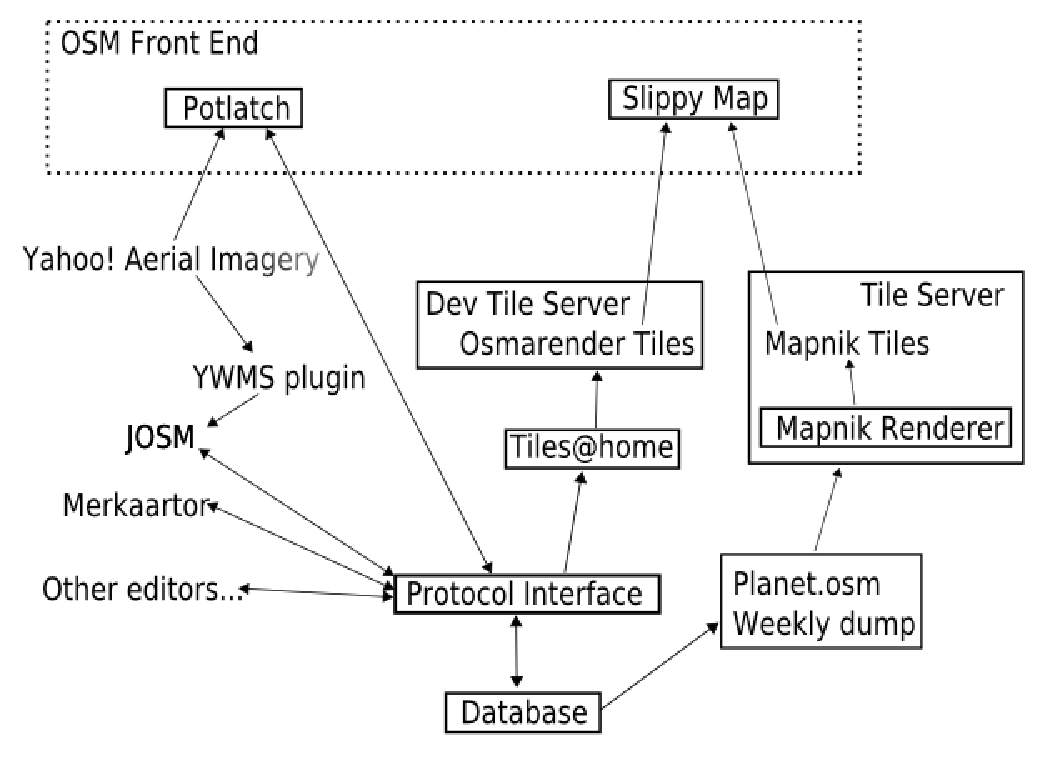
\includegraphics[height=4.5cm]{images/struttura.eps}
            \end{center}
        \end{frame}

        \begin{frame}
        \vspace{1.5cm}
        \begin{center}
            \begin{huge}\textbf{TeleAtlas: una pensa e 100 ne fa...}\end{huge}\\
            \begin{footnotesize}\textbf{...di errori!}
            \end{footnotesize}
        \end{center}
        \end{frame}

        \begin{frame}
            \vspace{1cm}
            \begin{center}
                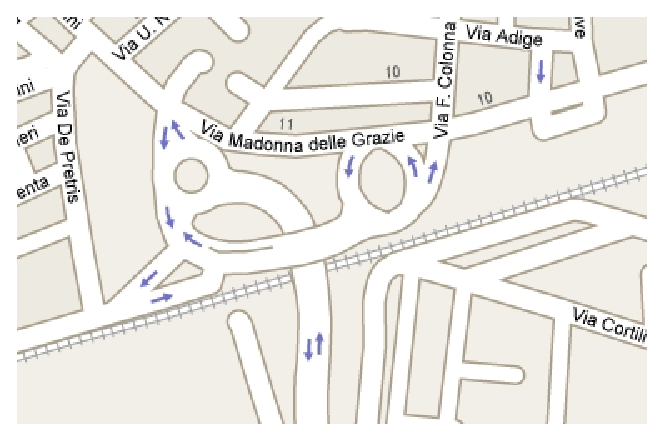
\includegraphics[height=5.5cm]{images/mappe/sottopasso.eps}
            \end{center}
        \end{frame}

        \begin{frame}{Immagini shock}
            \begin{center}
                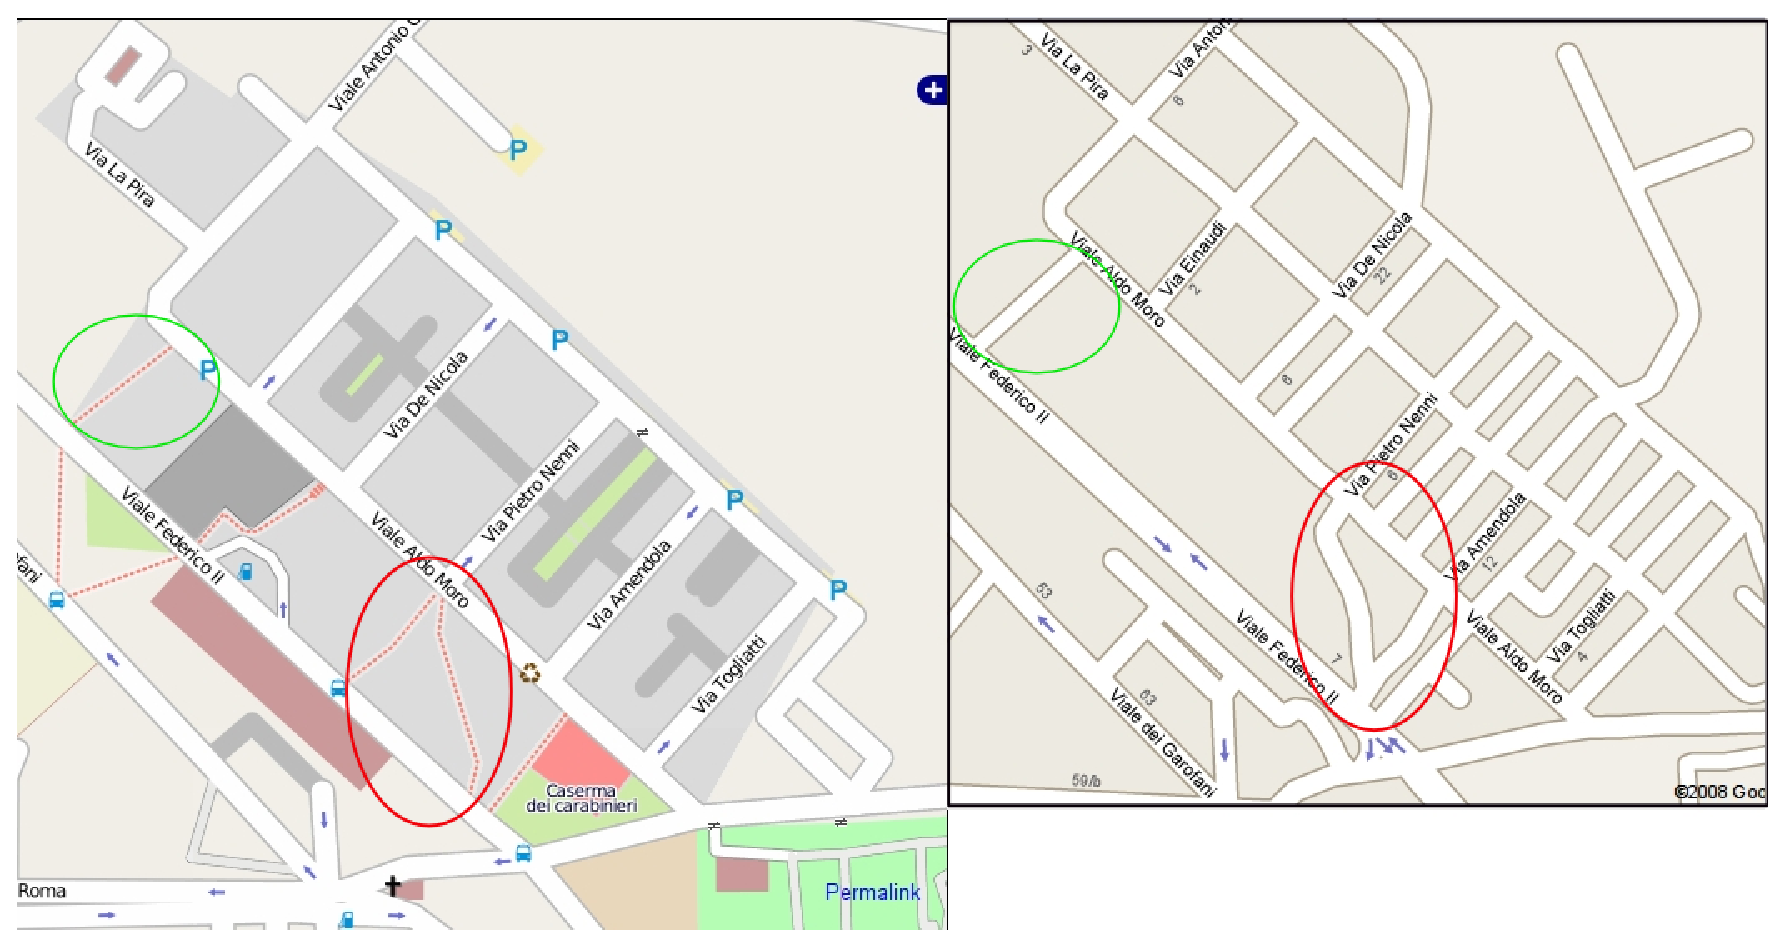
\includegraphics[height=5.5cm]{images/mappe/casafra.eps}
            \end{center}
        \end{frame}

        \begin{frame}{Immagini shock}
            \begin{center}
                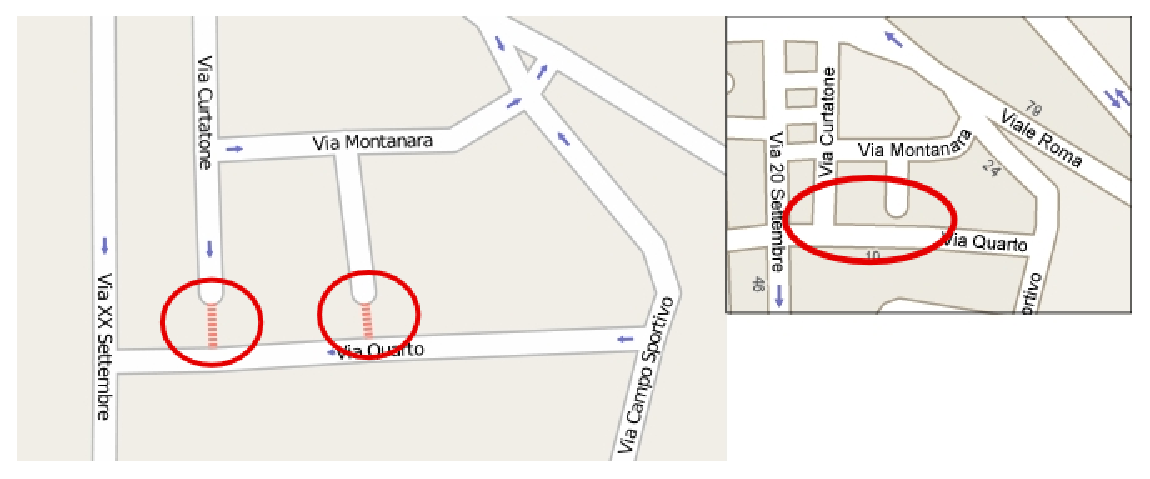
\includegraphics[height=4cm]{images/mappe/montanara.eps}
            \end{center}
        \end{frame}

        \begin{frame}{Immagini shock}
            \begin{center}
                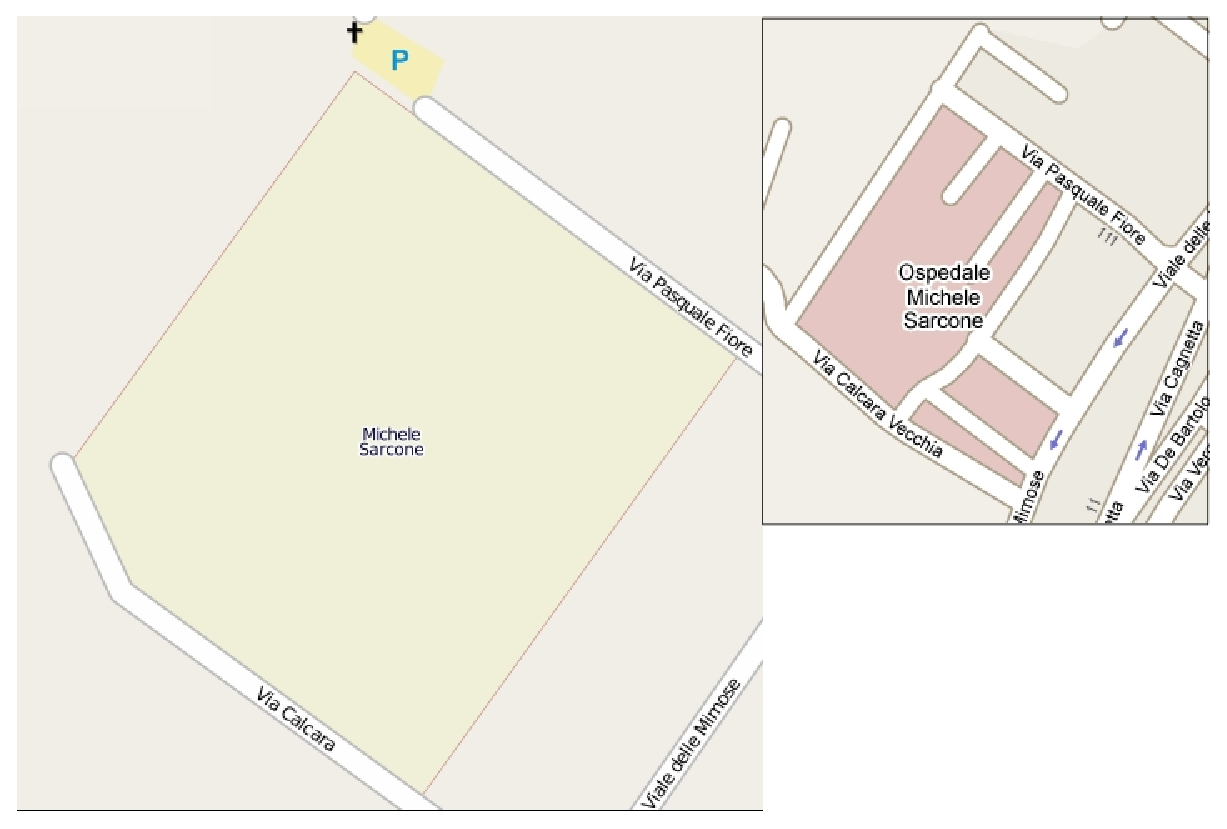
\includegraphics[height=5.5cm]{images/mappe/ospedale.eps}
            \end{center}
        \end{frame}

        \begin{frame}{Immagini shock}
            \begin{center}
                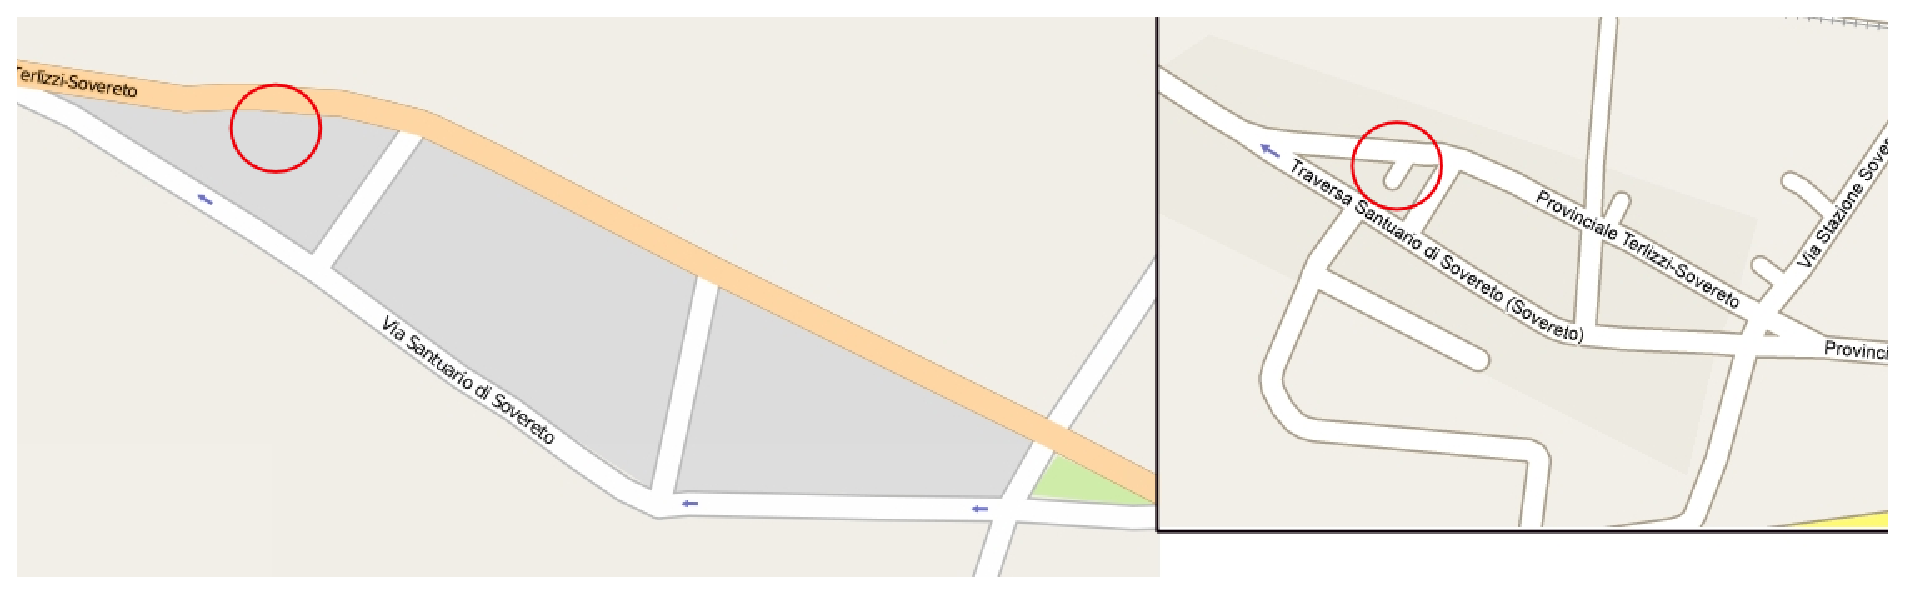
\includegraphics[height=3.5cm]{images/mappe/sovereto.eps}
            \end{center}
        \end{frame}

        \begin{frame}{Immagini shock}
            \begin{center}
                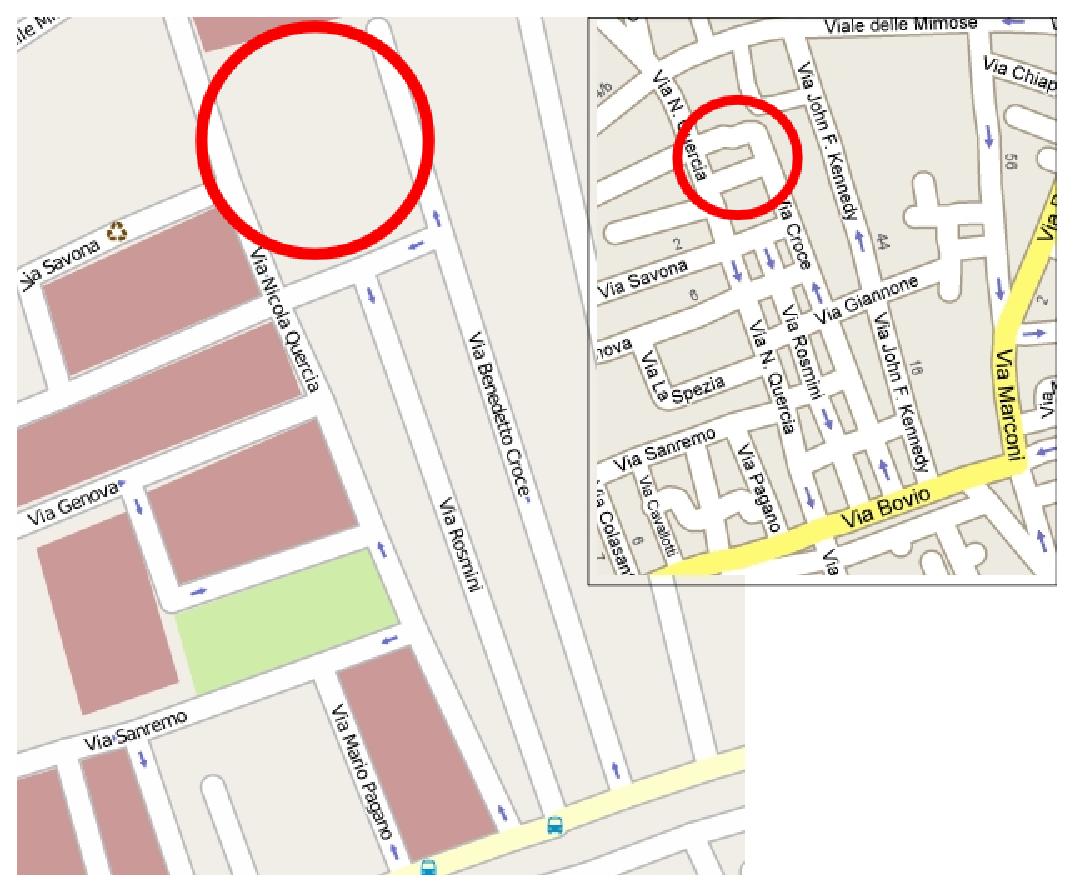
\includegraphics[height=6.5cm]{images/mappe/croce.eps}
            \end{center}
        \end{frame}

        \begin{frame}{Immagini shock}
            \vspace{1cm}
            \begin{center}
                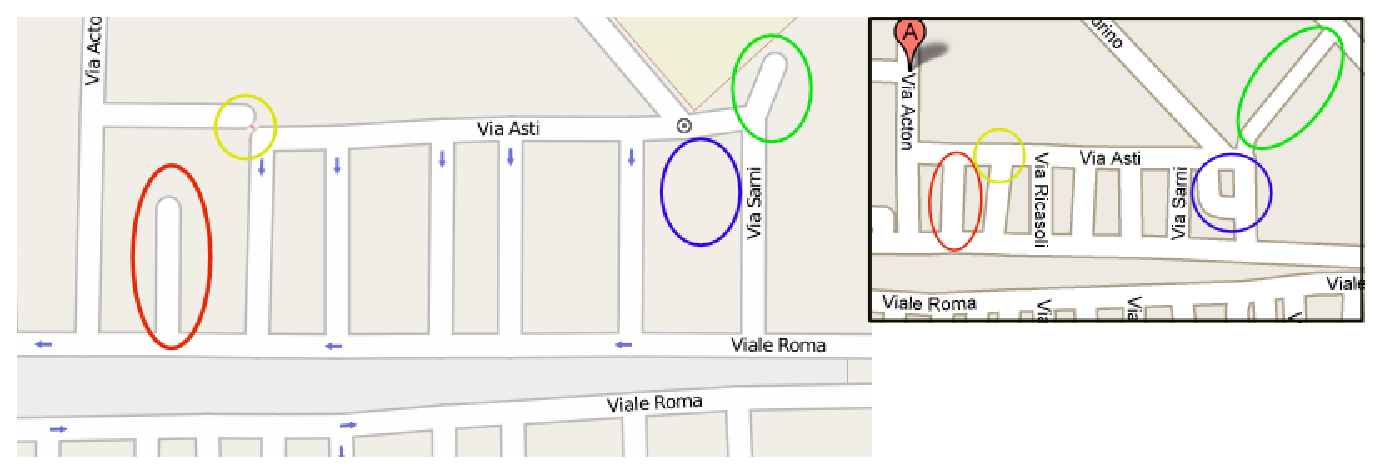
\includegraphics[height=3.5cm]{images/mappe/acton.eps}
            \end{center}
        \end{frame}

        \begin{frame}
        \vspace{1cm}
            \begin{center}
                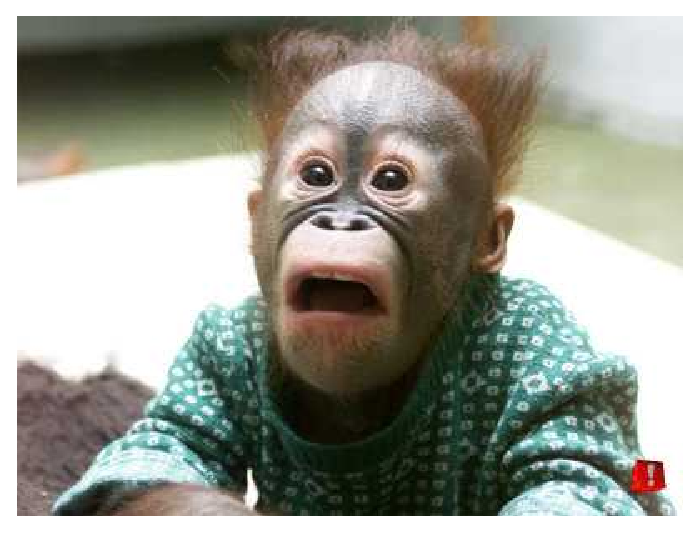
\includegraphics[height=5.5cm]{images/mappe/monkey.eps}
            \end{center}
        \end{frame}

        \begin{frame}{In bici a Roma...}
            \begin{center}
                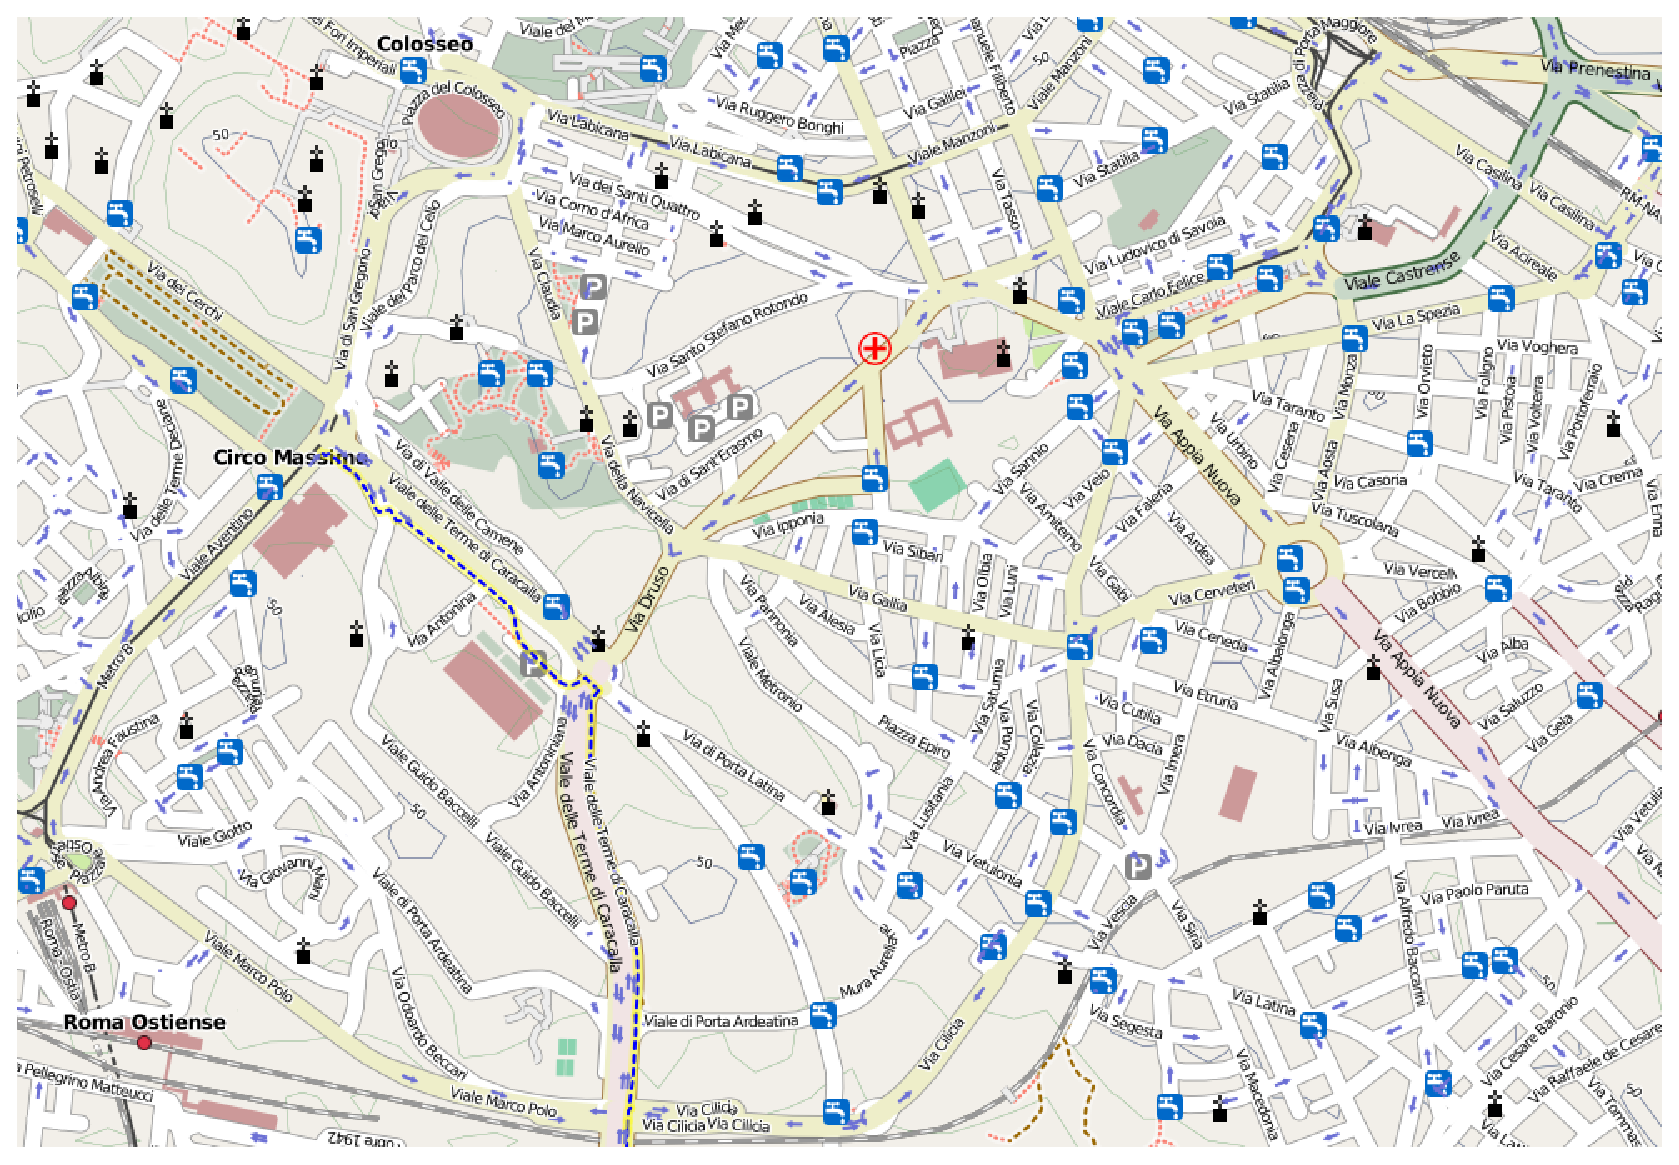
\includegraphics[height=6.5cm]{images/mappe/roma.eps}
            \end{center}
        \end{frame}

        \begin{frame}{Con gli sci sulle Alpi}
            \begin{center}
                \includegraphics[height=6cm]{images/openpiste.eps}
            \end{center}
        \end{frame}

        \begin{frame}{Dove Google non arriva...}
            \begin{center}
                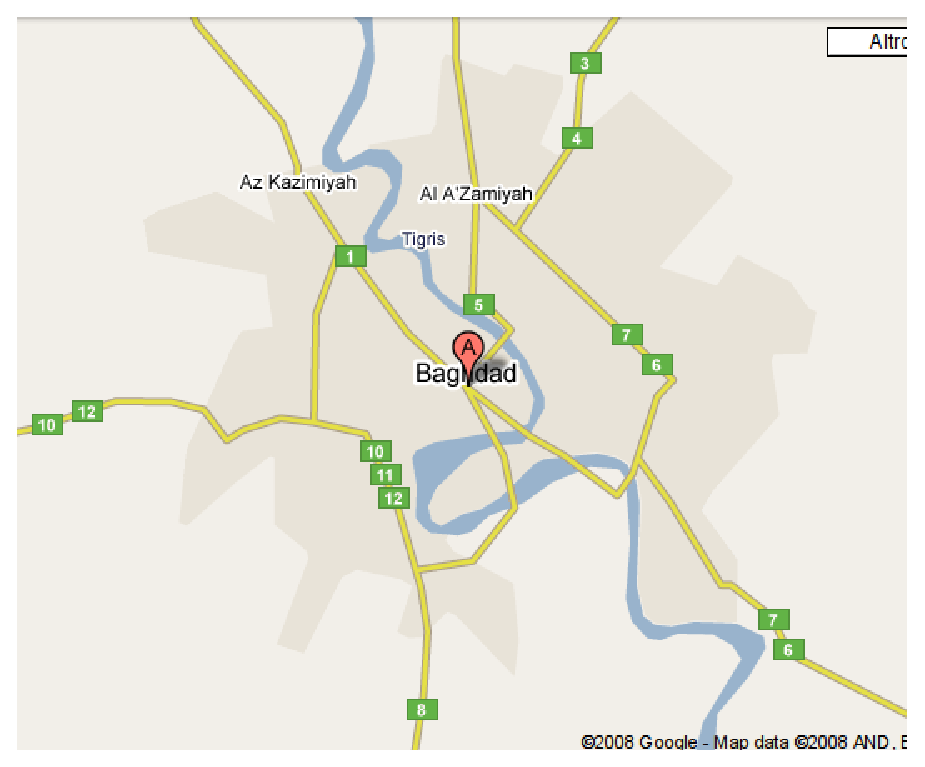
\includegraphics[height=6.5cm]{images/mappe/baghdadgoogle.eps}
            \end{center}
        \end{frame}

        \begin{frame}{Dove Google non arriva...}
            \begin{center}
                \includegraphics[height=6.5cm]{images/mappe/baghdad.eps}
            \end{center}
        \end{frame}

        \begin{frame}{Breve storia di OpenStreetMap}
            \begin{itemize}
                \item Agosto 2004: un'idea di Steve Coast (UK)
                \pause \item Gennaio 2006: nasce l'editor JOSM
                \pause \item Settembre 2007: inizia l'importazione dei dati \textit{TIGER}
                \pause \item Settembre 2007: \textit{Automotive Navigation Data} contribuisce Olanda, India e Cina
                \pause \item Maggio 2008:
                \begin{itemize}
                    \item 68.000 utenti iscritti, 3400 attivi per settimana (40.000/2.200 a giugno)
                    \item 510.000.000 di punti GPS (350.000.000 a giugno)
                \end{itemize}
            \end{itemize}
        \end{frame}

        \begin{frame}{Ulteriori informazioni}
            Per ulteriori informazioni:
            \begin{Large}
                \begin{center}
                    www.openstreetmap.org\\
                    http://wiki.openstreetmap.org\vspace{1cm}\\
                    www.openlayers.org\\
                    http://fradeve.netsons.org\\
                    http://sdonk.netsons.org\\
                \end{center}
            \end{Large}
        \end{frame}

        \begin{frame}{Credits}
            Si ringrazia per il supporto:\\
            \begin{center}
                LUGBari (www.lugbari.org)\\
                Simone Cortesi (OpenStreetMap.it)\\
            \end{center}
            \begin{center}
                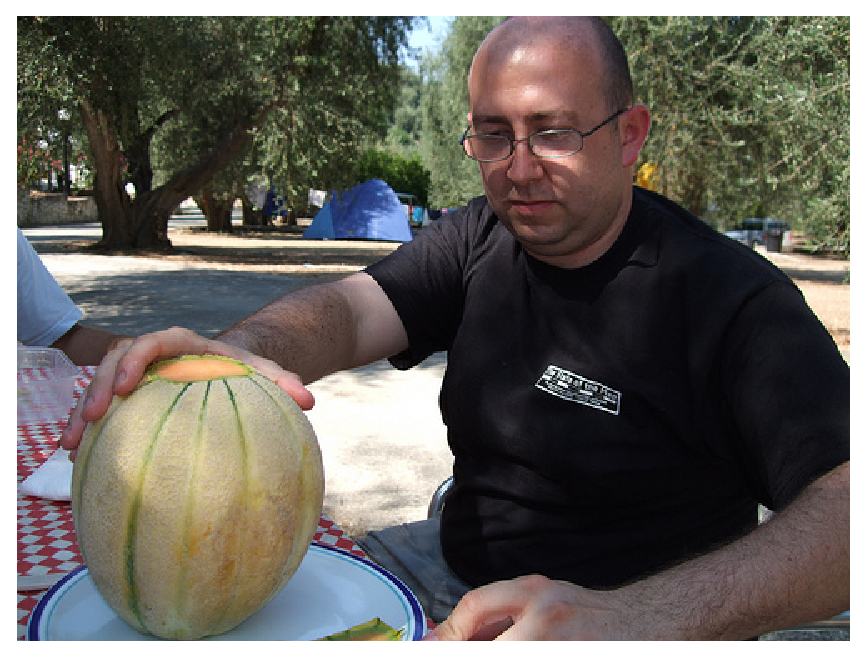
\includegraphics[height=5.5cm]{images/simone.eps}
            \end{center}
        \end{frame}

\end{document}
